\begin{figure}[H]
\centering
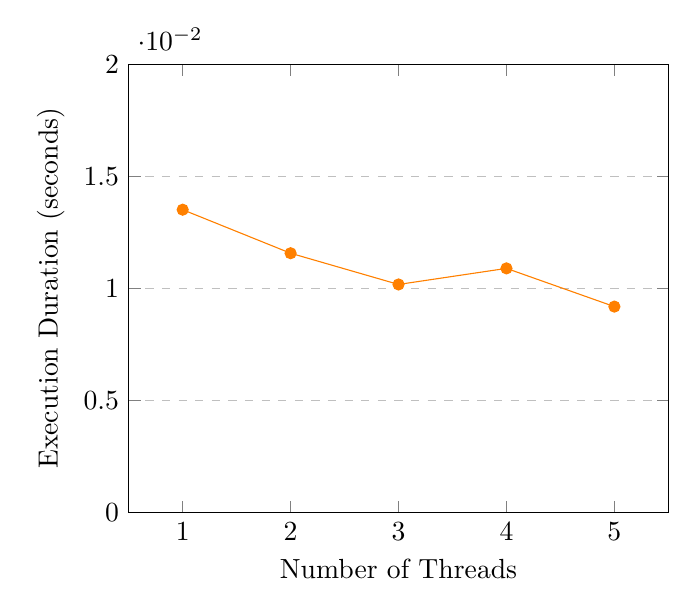
\begin{tikzpicture}
\begin{axis}[
    xlabel={Number of Threads},
    ylabel={Execution Duration (seconds)},
    xmin=0.5, xmax=5.5,
    ymin=0, ymax=0.02,
    xtick={1, 2, 3, 4, 5},
    ytick={0, 0.005, 0.01, 0.015, 0.02},
    ymajorgrids=true,
    grid style=dashed,
]
\addplot[
    color=orange,
    mark=*,
    ]
    coordinates {
    (1,0.013509184) (2,0.011566795) (3,0.010173890) (4,0.010891230) (5,0.009185814)
    };

\end{axis}
\end{tikzpicture}
\caption{Execution Duration vs. Number of Threads for Circle}
\label{fig:circle}
\end{figure}